\Chapter{1}
\section*{基礎データ取得実験結果}
基礎データ取得実験にて得られた結果を示す。
本実験において加圧ガスであるGHeの圧力がバルブ解放直後、一時的に振動を起こし、
直後に振動が収束するケースがある、一方振動が収束せず、実験中も振動し続けるケースもあった。
安定して計測できないケースは解析には使用していない。
一方下流部に位置するインジェクタ上流部圧力は正常に動作しており、GHe圧力との関係はわからなかった。
この振動についてFFTをかけてみたが、特に目立つ振動数は確認できず、振動の原因を特定することができなかった。
温度の時間履歴についてはすべてのケースにおいて安定して計測することができた。
今回の実験では極低温物体の温度計測を行うため、大気圧下での液体酸素による温度校正を行った。
一部実験中に熱電対が焼損し温度計測が出来ていないものがある。使用した熱電対はk型熱電対で計測可能上限が1400Kまでであり、
使用可能範囲を超えていたことから、焼き切れたと考えている。
ハイブリッドロケットエンジンにおいて液体酸素が気化する過程で発生する低周波数の振動がよく観測される。
本実験において各圧力及び流量にスペクトログラムをかけて観測してみたが、
低周波成分の振動は観測できず、また振動がシフトしていく様子もなかった。
今回の実験機は非常に小型なものであり、また流量も非常に低いので、特に目立つ周波数成分は観測できなかったが、
今後スケールアップしていく上で障害になる可能性がある。
\newcommand{\FigAddApp}{./src/Appendix/Figure}
\begin{figure}
\centering
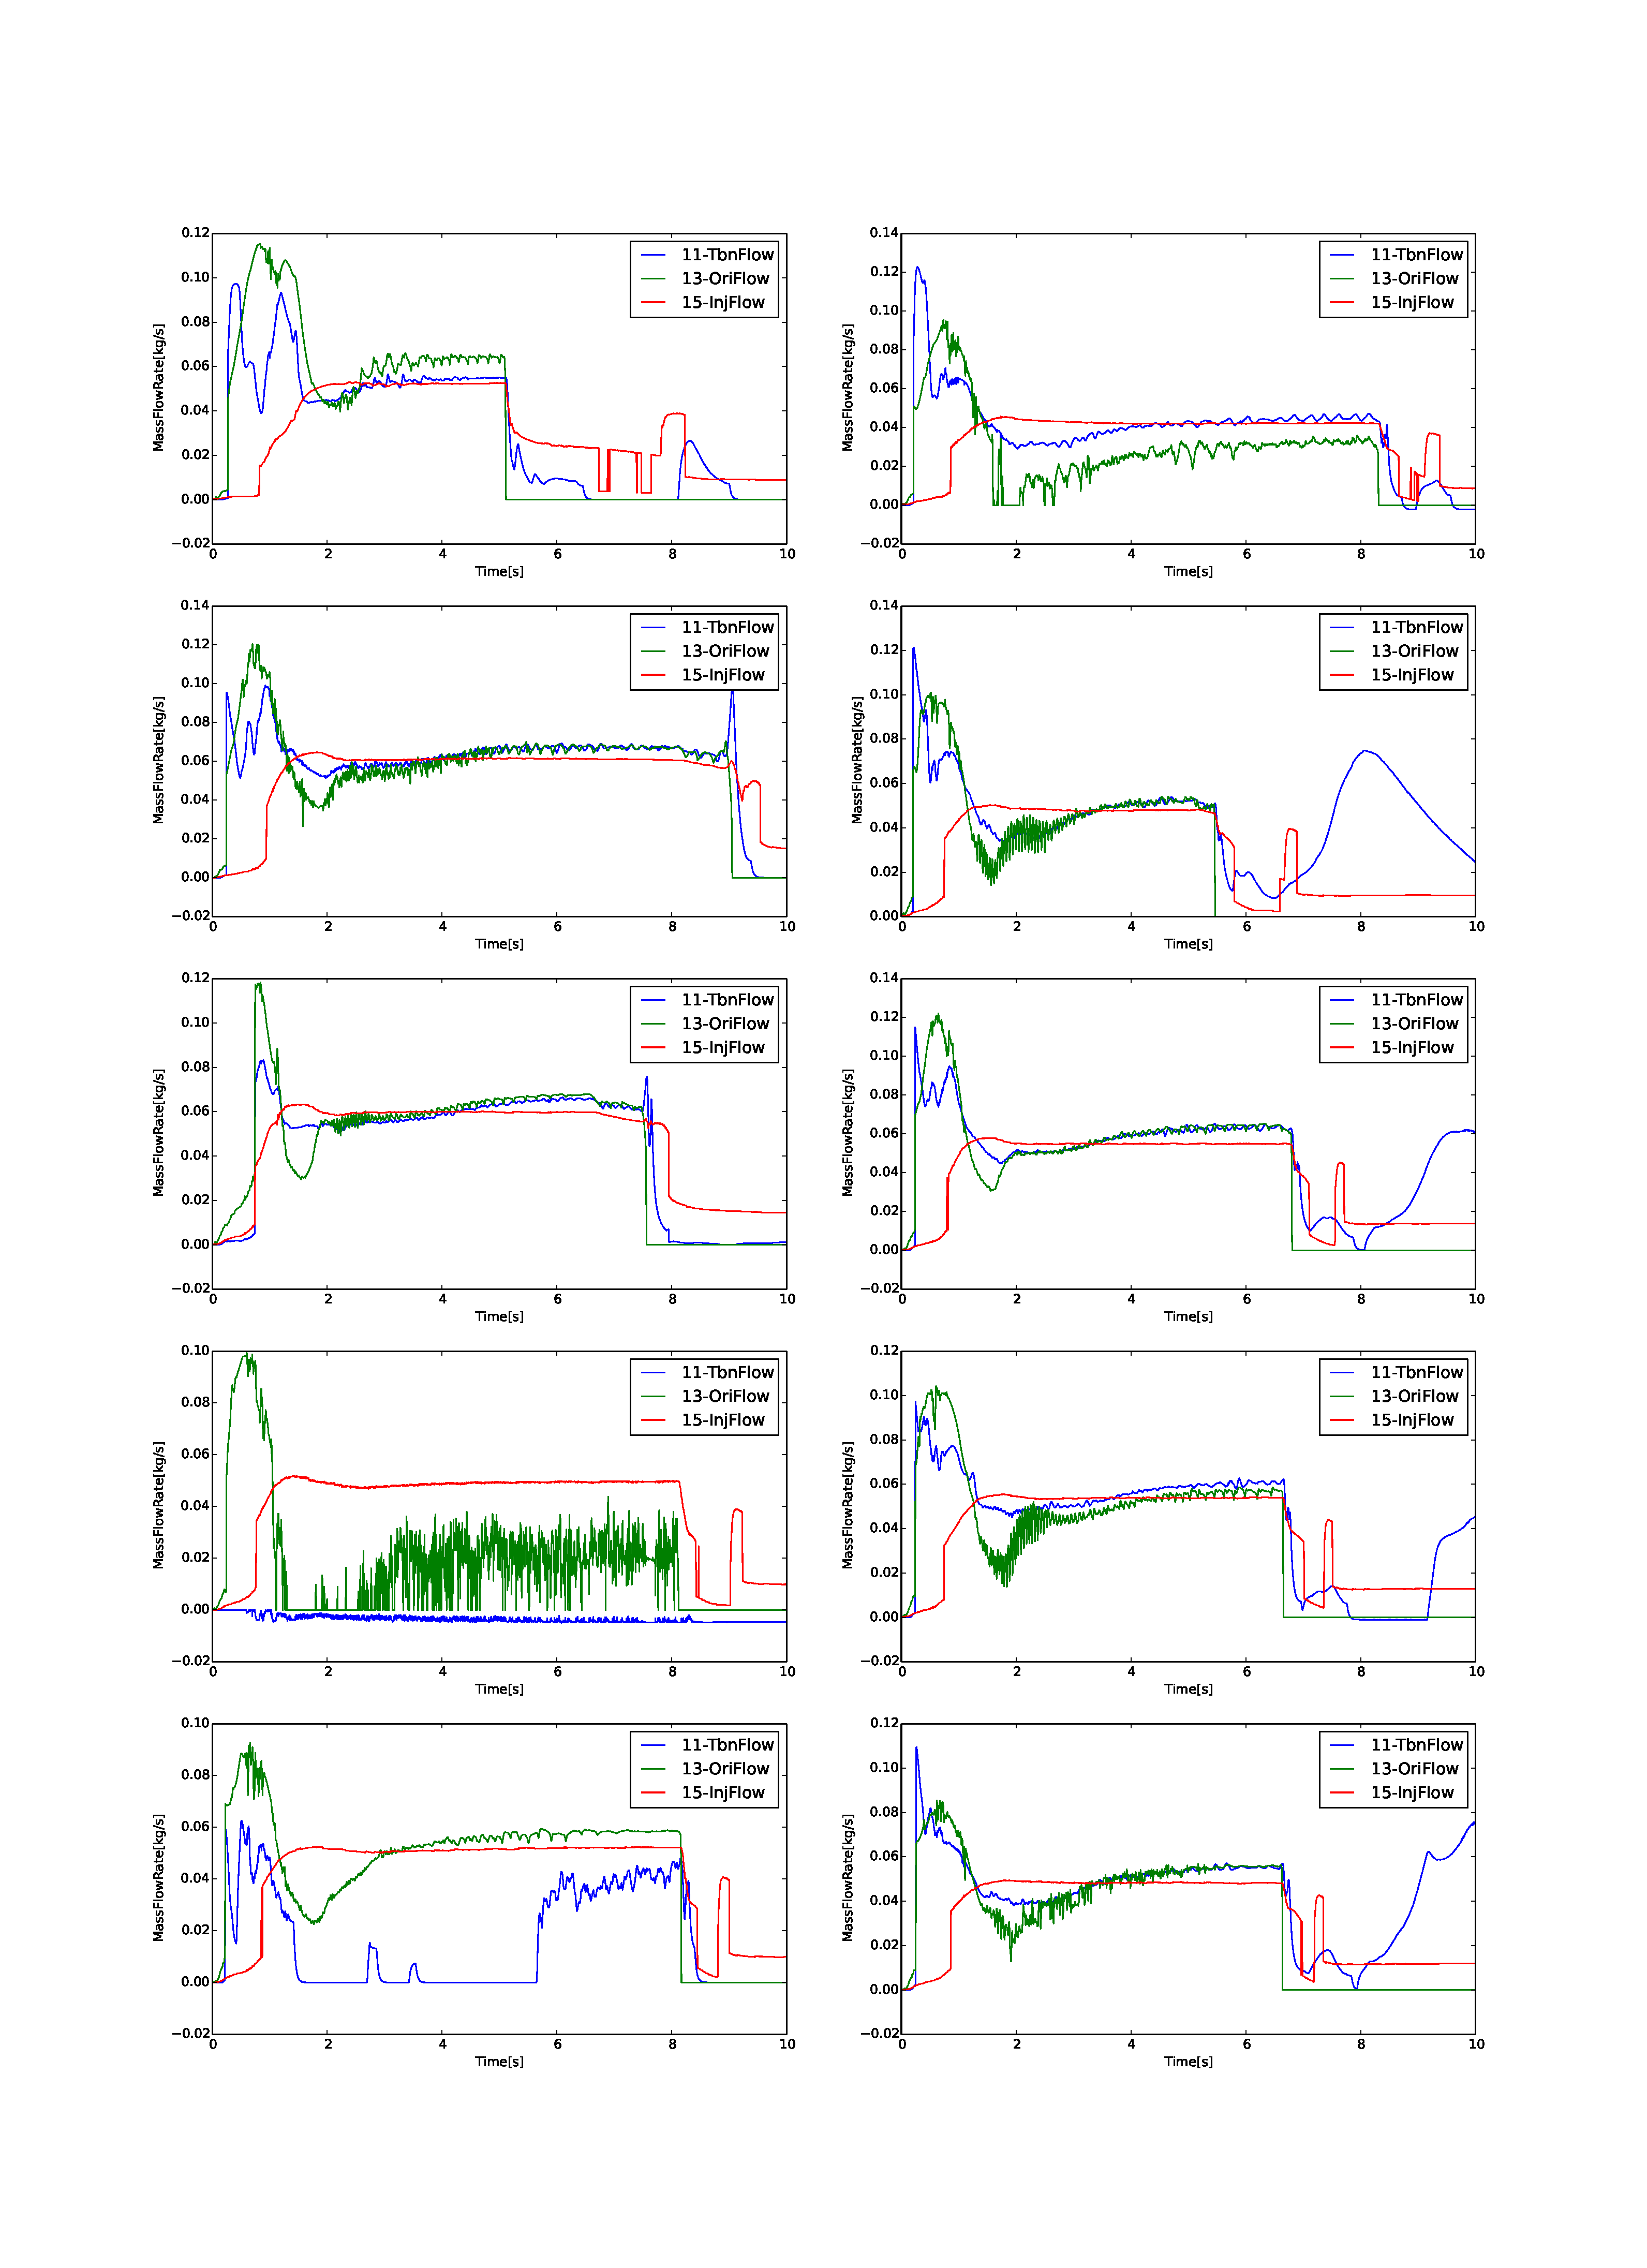
\includegraphics[width=14cm]{\FigAddApp/History/MassFlow.eps}
\caption{}
\end{figure}
\begin{figure}
\centering
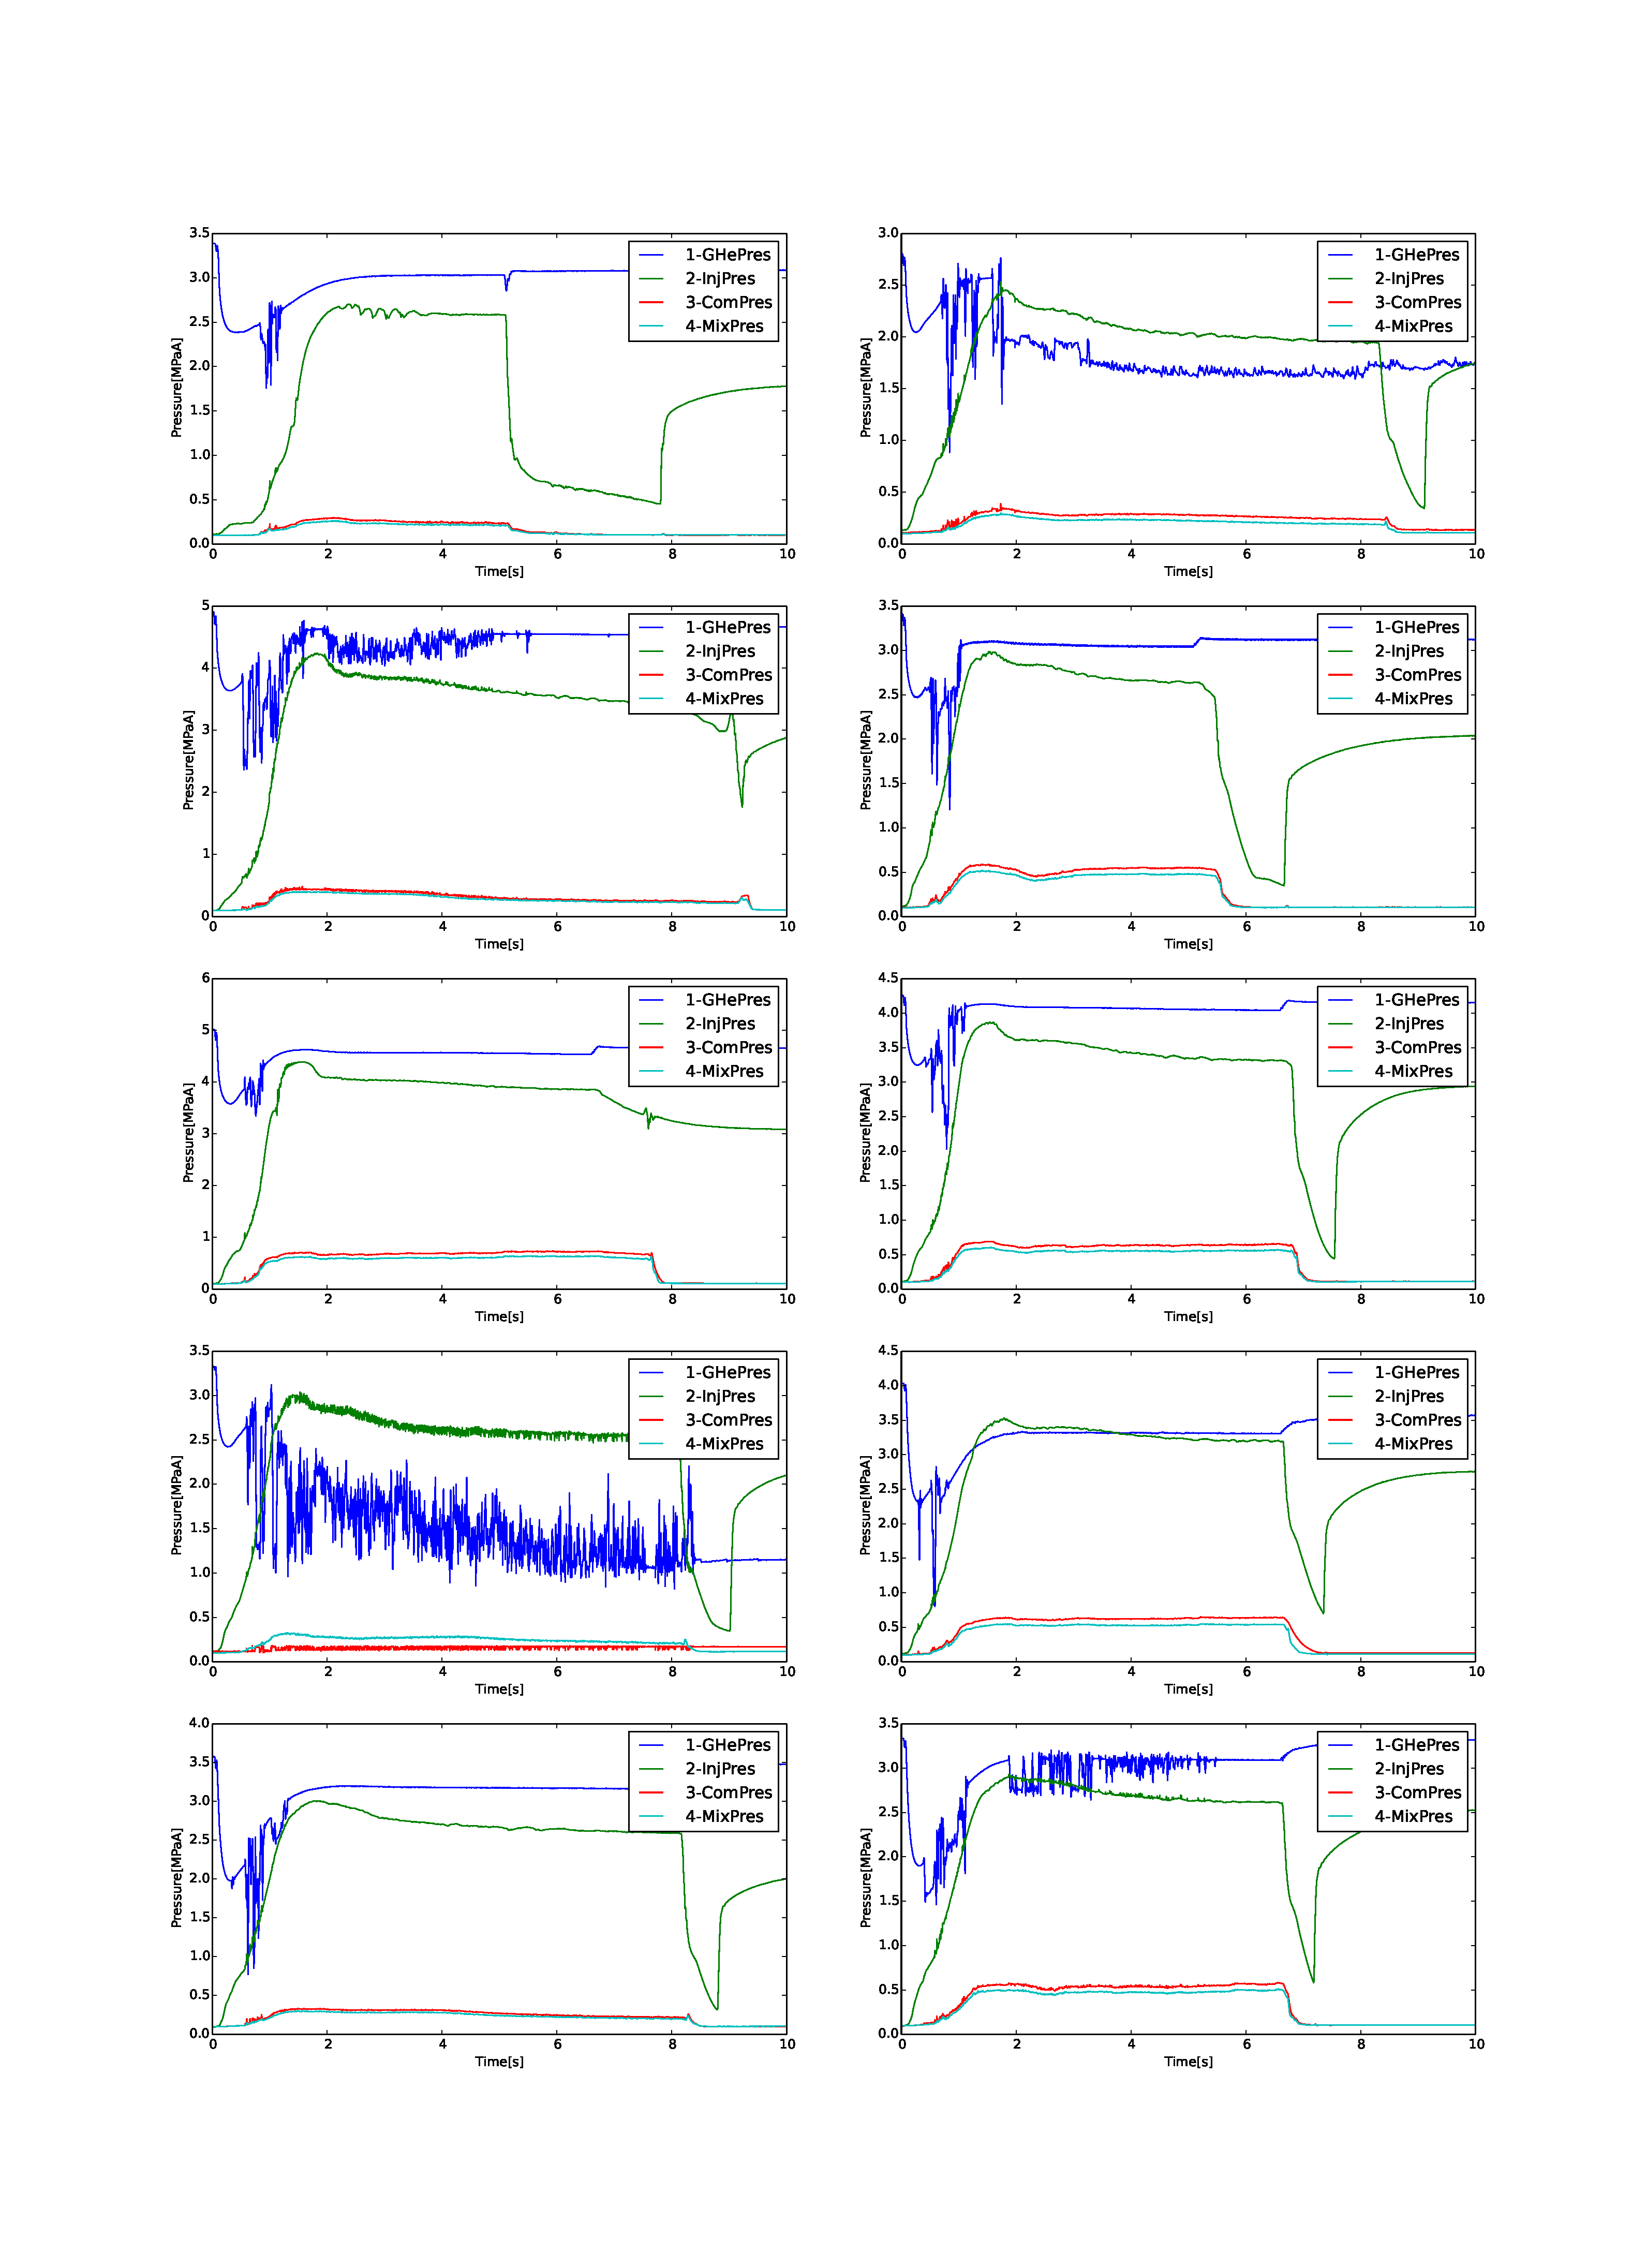
\includegraphics[width=14cm]{\FigAddApp/History/Pressure.eps}
\caption{}
\end{figure}
\begin{figure}
\centering
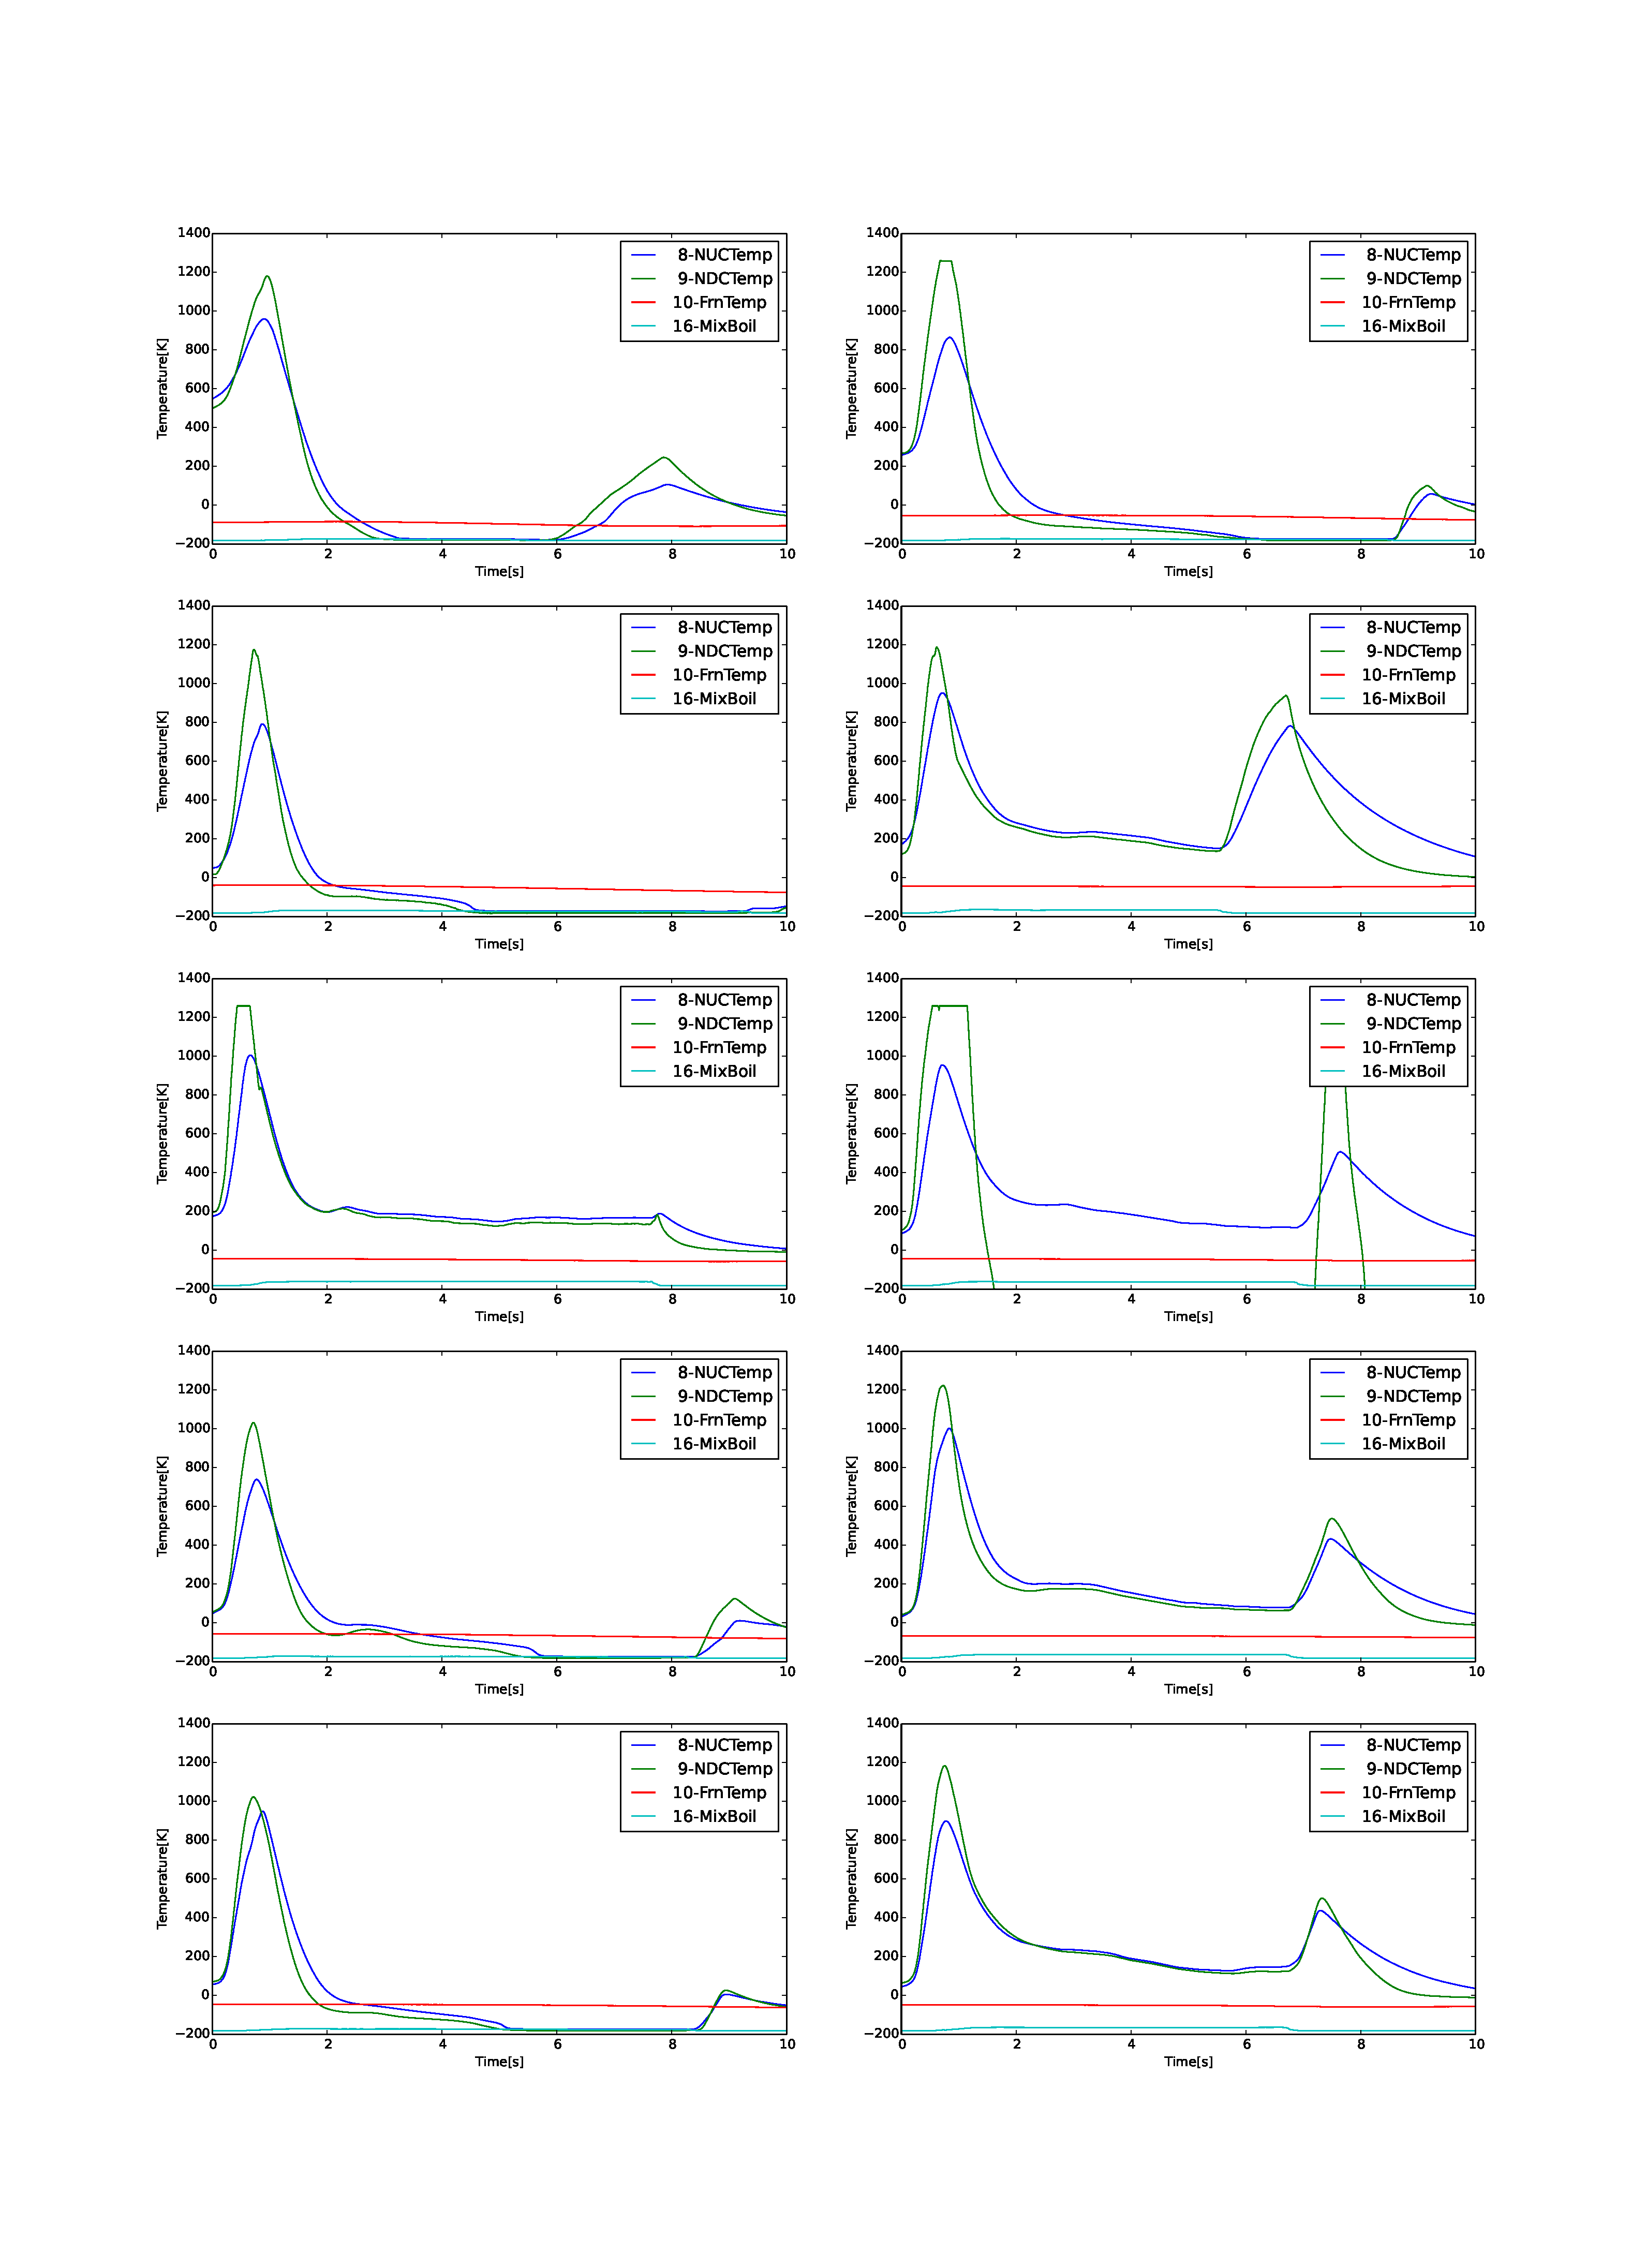
\includegraphics[width=14cm]{\FigAddApp/History/Temperature.eps}
\caption{}
\end{figure}
\begin{figure}
\centering
\includegraphics[width=14cm]{\FigAddApp/SpecGram/1-GHePres.eps}
\caption{}
\end{figure}
\begin{figure}
\centering
\includegraphics[width=14cm]{\FigAddApp/SpecGram/2-InjPres.eps}
\caption{}
\end{figure}
\begin{figure}
\centering
\includegraphics[width=14cm]{\FigAddApp/SpecGram/3-ComPres.eps}
\caption{}
\end{figure}
\begin{figure}
\centering
\includegraphics[width=14cm]{\FigAddApp/SpecGram/4-MixPres.eps}
\caption{}
\end{figure}
\begin{figure}
\centering
\includegraphics[width=14cm]{\FigAddApp/SpecGram/11-TbnFlow.eps}
\caption{}
\end{figure}
